% !TEX program = xelatex
\documentclass[a4paper,10pt]{article}

\makeatletter
\let\@expl@@@mark@update@singlecol@structures@@\relax
\makeatother

\usepackage[a4paper, left=0.95cm, right=0.95cm, top=0.80cm, bottom=0.90cm, footskip=0.48cm]{geometry}
\usepackage{fontspec}
\usepackage{amsmath, amssymb}
\usepackage{array, colortbl, tabularx}
\usepackage[table]{xcolor}
\usepackage{tcolorbox}
\tcbuselibrary{skins}
\usepackage{fancyhdr}
\usepackage{enumitem}
\usepackage{tikz}
\usetikzlibrary{calc, angles, quotes, arrows.meta}

% Cross-platform font discovery
\makeatletter
\newcommand{\NGSFindFonts}{%
  \IfFileExists{../../../fonts/KhmerOSsiemreap.ttf}{%
    \def\NGSUserPath{../../../fonts/}\def\NGSSysPath{../../../fonts/}%
  }{%
    \IfFileExists{../../../../fonts/KhmerOSsiemreap.ttf}{%
      \def\NGSUserPath{../../../../fonts/}\def\NGSSysPath{../../../../fonts/}%
    }{%
      \IfFileExists{fonts/KhmerOSsiemreap.ttf}{%
        \def\NGSUserPath{fonts/}\def\NGSSysPath{fonts/}%
      }{%
        \def\NGSUserPath{C:/Users/user/AppData/Local/Microsoft/Windows/Fonts/}%
        \def\NGSSysPath{C:/Windows/Fonts/}%
      }%
    }%
  }%
}
\NGSFindFonts
\makeatother

\XeTeXlinebreaklocale "km"
\XeTeXlinebreakskip = 0pt plus 1pt minus 0.1pt

\setmainfont[
  Path = {\NGSUserPath},
  Extension = .ttf,
  UprightFont = KhmerOSsiemreap,
  BoldFont = KhmerOSsiemreap,
  BoldFeatures = {FakeBold=1.8},
  ItalicFont = KhmerOSsiemreap,
  ItalicFeatures = {FakeSlant=0.25}
]{KhmerOSsiemreap}

\newfontfamily\muol[Path={\NGSUserPath}]{KhmerOSmuollight.ttf}
\newfontfamily\enfont[Path={\NGSSysPath}, Scale=1.0]{times.ttf}
\newfontfamily\enbold[Path={\NGSSysPath}, Scale=1.0]{timesbd.ttf}
\newfontfamily\calibrifont[Path={\NGSSysPath}, Scale=0.95]{calibri.ttf}

\DeclareTextFontCommand{\en}{\enfont}
\newcommand{\enbf}[1]{{\enbold #1}}

\definecolor{headgray}{HTML}{E2E2E2}
\definecolor{panelgray}{HTML}{F5F5F5}

\pagestyle{fancy}
\fancyhf{}
\renewcommand{\headrulewidth}{0pt}
\renewcommand{\footrulewidth}{0.4pt}
\fancyfoot[L]{\fontsize{8.5pt}{11pt}\selectfont អនុវិទ្យាល័យព្រះក្រសាំង $\;\vert\;$ គណិតវិទ្យា ថ្នាក់ទី៨ $\;\vert\;$ មេរៀនទី១៥ (១៥.២.៣) លក្ខណៈឆ្លុះនៃរង្វង់ និងលំហាត់សំយោគ}
\fancyfoot[R]{\fontsize{8.5pt}{11pt}\selectfont ទំព័រ \en{\thepage/2}}

\setlength{\parindent}{0pt}
\setlength{\tabcolsep}{4pt}

\newcommand{\tri}[1]{\triangle #1}
\newcommand{\unit}[1]{\,\text{\en{#1}}}
\newcommand{\blank}[1]{\leavevmode\hbox to #1{\dotfill}}
\newcommand{\chkbox}{\tikz[baseline=-0.3ex]\draw[black, line width=0.65pt] (0,0) rectangle (0.27cm,0.27cm);}
\newcommand{\cnum}[1]{\tikz[baseline=-0.58ex]\node[circle, fill=black, text=white, inner sep=0.85pt, minimum size=1.95ex, font=\enbold\scriptsize]{#1};}

\newcommand{\arc}[1]{\mbox{%
  \tikz[baseline=(arcX.base)]{%
    \node[inner sep=0pt, outer sep=0pt] (arcX) {$#1$};%
    \draw[black, line width=0.55pt] ($(arcX.north west)+(0.02,0.035)$) to[bend left=30] ($(arcX.north east)+(-0.02,0.035)$);%
  }%
}}

\newcommand{\tickone}[2]{%
  \coordinate (tkM) at ($(#1)!0.5!(#2)$);
  \draw[black, line width=0.7pt] ($(tkM)!0.10cm!90:(#2)$) -- ($(tkM)!0.10cm!-90:(#2)$);
}
\newcommand{\ticktwo}[2]{%
  \coordinate (tkM1) at ($(#1)!0.47!(#2)$);
  \coordinate (tkM2) at ($(#1)!0.53!(#2)$);
  \draw[black, line width=0.7pt] ($(tkM1)!0.10cm!90:(#2)$) -- ($(tkM1)!0.10cm!-90:(#2)$);
  \draw[black, line width=0.7pt] ($(tkM2)!0.10cm!90:(#2)$) -- ($(tkM2)!0.10cm!-90:(#2)$);
}

\newcommand{\secbar}[2]{%
  \vspace{2.5pt}%
  \begin{tcolorbox}[
    enhanced, sharp corners, colback=headgray, colframe=black,
    boxrule=0.75pt, left=5pt, right=5pt, top=2.5pt, bottom=2.5pt,
    before skip=2pt, after skip=3pt
  ]
    {\muol\fontsize{9.6pt}{14pt}\selectfont #1}\hfill{\fontsize{9pt}{13pt}\selectfont\textbf{#2}}
  \end{tcolorbox}%
}

\begin{document}
\fontsize{9.6pt}{14.2pt}\selectfont

% ==================== ក្បាលសន្លឹកកិច្ចការ ====================
\begin{tcolorbox}[
  enhanced, sharp corners, colback=white, colframe=black,
  boxrule=0.95pt, left=6pt, right=6pt, top=3.5pt, bottom=3.5pt, after skip=3pt
]
  \begin{minipage}[c]{11.2cm}
    {\muol\fontsize{10.5pt}{15.5pt}\selectfont សន្លឹកកិច្ចការសិស្ស — មេរៀនទី១៥ ៖ រង្វង់}\\[1.5pt]
    \textbf{ចំណុច ២.២ ៖ លក្ខណៈឆ្លុះនៃរង្វង់ និងលំហាត់សំយោគ} (សៀវភៅគោល ទំ.២០២--២០៤)
  \end{minipage}\hfill
  \begin{minipage}[c]{6.7cm}
    ឈ្មោះសិស្ស៖ \blank{4.4cm}\\[2pt]
    ថ្នាក់ទី៨៖ \blank{1.3cm} \hspace{0.2cm} ដៃគូទី៖ \blank{2.0cm}
  \end{minipage}
\end{tcolorbox}

% ==================== ផ្នែកទី ១ ៖ E1 - ENGAGE ====================
\secbar{ផ្នែកទី ១ ៖ បេសកកម្មជាងសំណង់ (\enbf{E1}) — ទទឹងផ្ទៃទឹកក្នុងលូបេតុងមូល}{\en{3} នាទី (ទស្សន៍ទាយមុនរៀន)}

\begin{tcolorbox}[
  enhanced, sharp corners, colback=panelgray, colframe=black,
  boxrule=0.8pt, left=6pt, right=6pt, top=3pt, bottom=3pt, after skip=3pt
]
  \begin{minipage}[c]{12.4cm}\raggedright
    ជាងសំណង់ពិនិត្យមុខកាត់ទទឹងនៃ \textbf{លូបេតុងមូល} មួយដែលមានកាំក្នុង $r = 5\unit{dm}$។ ពេលទឹកហូរ ផ្ទៃទឹកបង្កើតបានជាអង្កត់ធ្នូដេក $CD$ ស្ថិតនៅចម្ងាយកែង $OH = 3\unit{dm}$ ក្រោមផ្ចិត $O$។ ចូរទស្សន៍ទាយ៖\\[2pt]
    ១. តើ $AB \perp CD$ ចែក $CD$ ស្មើគ្នាឬទេ? \hspace{0.15cm} \mbox{\chkbox\ ចែកស្មើគ្នា ($HC=HD$)} \hspace{0.2cm} \mbox{\chkbox\ មិនស្មើគ្នា}\\[2pt]
    ២. តើទទឹងផ្ទៃទឹក $CD$ ស្មើប៉ុន្មាន? \hspace{0.15cm} \mbox{\chkbox\ $4\unit{dm}$} \hspace{0.22cm} \mbox{\chkbox\ $8\unit{dm}$} \hspace{0.22cm} \mbox{\chkbox\ $10\unit{dm}$}
  \end{minipage}\hfill
  \begin{minipage}[c]{5.6cm}
    \centering
    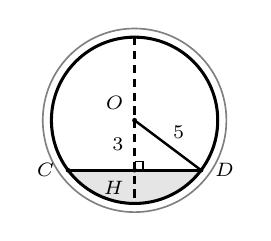
\begin{tikzpicture}[scale=0.44, every node/.style={font=\scriptsize, text=black}]
      \coordinate (O) at (0,0);
      \def\R{2.4}
      \def\yH{-1.44}
      \def\xC{1.92}
      \coordinate (A) at (0,\R);
      \coordinate (B) at (0,-\R);
      \coordinate (H) at (0,\yH);
      \coordinate (C) at (-\xC,\yH);
      \coordinate (D) at (\xC,\yH);
      \draw[black!50, line width=0.6pt] (O) circle (2.65);
      \begin{scope}
        \clip (O) circle (\R);
        \fill[black!10] (-2.5,-2.5) rectangle (2.5,\yH);
      \end{scope}
      \draw[black, line width=1.1pt] (O) circle (\R);
      \draw[black, line width=1.1pt] (C)--(D);
      \draw[black, line width=0.8pt, densely dashed] (A)--(B);
      \draw[black, line width=0.9pt] (O)--(D);
      \draw[black, line width=0.65pt] ($(H)+(0,0.25)$) -- ($(H)+(0.25,0.25)$) -- ($(H)+(0.25,0)$);
      \fill[black] (O) circle (2pt) (H) circle (1.9pt) (C) circle (1.9pt) (D) circle (1.9pt);
      \node[above left=0.5pt] at (O) {$O$};
      \node[below left=0.5pt] at (H) {$H$};
      \node[left=1.5pt] at (C) {$C$};
      \node[right=1.5pt] at (D) {$D$};
      \node[left=0.5pt] at (0,-0.70) {$3$};
      \node[above right=-1.5pt] at (0.95,-0.70) {$5$};
    \end{tikzpicture}
  \end{minipage}
\end{tcolorbox}

% ==================== ផ្នែកទី ២ ៖ E2 - EXPLORE ====================
\secbar{ផ្នែកទី ២ ៖ រុករកផ្ចិតឆ្លុះ អ័ក្សឆ្លុះ និងអង្កត់ផ្ចិតកែងនឹងអង្កត់ធ្នូ (\enbf{E2 — Explore})}{\en{11} នាទី (ពិភាក្សាដៃគូ)}

\begin{minipage}[c]{6.4cm}
  \centering
  \begin{tikzpicture}[scale=0.38, every node/.style={font=\scriptsize, text=black}]
    % រូបក៖ ផ្ចិតឆ្លុះ និងអ័ក្សឆ្លុះ (ទំ.២០២)
    \begin{scope}[shift={(0,0)}]
      \coordinate (O) at (2.3,2.5);
      \def\R{2.0}
      \coordinate (P) at ($(O)+(55:\R)$);
      \coordinate (P1) at ($(O)+(-55:\R)$);
      \coordinate (Ps) at ($(O)+(235:\R)$);
      \coordinate (K) at ($(P)!(O)!(P1)$);
      \draw[black, line width=0.95pt] (O) circle (\R);
      \draw[black, line width=1.0pt] ($(O)+(-2.3,0)$) -- ($(O)+(2.3,0)$) node[right=0pt] {$d$};
      \draw[black, line width=0.8pt, densely dashed] (P)--(P1) (P)--(Ps);
      \draw[black, line width=0.6pt] ($(K)+(0,0.20)$)--($(K)+(-0.20,0.20)$)--($(K)+(-0.20,0)$);
      \tickone{O}{P}\tickone{O}{Ps}
      \ticktwo{P}{K}\ticktwo{K}{P1}
      \fill[black] (O) circle (2pt) (P) circle (1.9pt) (P1) circle (1.9pt) (Ps) circle (1.9pt) (K) circle (1.7pt);
      \node[above left=0.5pt] at (O) {$O$};
      \node[above right=0pt] at (P) {$B$};
      \node[below right=0pt] at (P1) {$B_1$};
      \node[below left=0pt] at (Ps) {$B'$};
      \node[align=center] at (2.3,-1.65) {(ក) ផ្ចិតឆ្លុះ $O$\\និងអ័ក្សឆ្លុះ $d$};
    \end{scope}
    % រូបខ៖ អង្កត់ផ្ចិត AB ⊥ CD (ទំ.២០៣)
    \begin{scope}[shift={(6.6,0)}]
      \coordinate (O2) at (2.3,2.5);
      \def\R{2.0}
      \coordinate (A2) at ($(O2)+(0,\R)$);
      \coordinate (B2) at ($(O2)+(0,-\R)$);
      \coordinate (C2) at ($(O2)+(-145:\R)$);
      \coordinate (D2) at ($(O2)+(-35:\R)$);
      \coordinate (H2) at ($(C2)!(O2)!(D2)$);
      \draw[black, line width=0.95pt] (O2) circle (\R);
      \draw[black, line width=1.0pt] (A2)--(B2) (C2)--(D2);
      \draw[black, line width=0.75pt, densely dashed] (O2)--(C2) (O2)--(D2);
      \draw[black, line width=0.6pt] ($(H2)+(0,0.20)$)--($(H2)+(0.20,0.20)$)--($(H2)+(0.20,0)$);
      \tickone{O2}{C2}\tickone{O2}{D2}
      \fill[black] (O2) circle (2pt) (A2) circle (1.9pt) (B2) circle (1.9pt) (C2) circle (1.9pt) (D2) circle (1.9pt) (H2) circle (1.8pt);
      \node[right=1pt] at (O2) {$O$};
      \node[above=0.5pt] at (A2) {$A$};
      \node[below=0.5pt] at (B2) {$B$};
      \node[below left=0pt] at (C2) {$C$};
      \node[below right=0pt] at (D2) {$D$};
      \node[above left=0pt] at (H2) {$H$};
      \node[align=center] at (2.3,-1.65) {(ខ) អង្កត់ផ្ចិត\\$AB \perp CD$ ត្រង់ $H$};
    \end{scope}
  \end{tikzpicture}
\end{minipage}\hfill
\begin{minipage}[c]{12.2cm}
  \textbf{ប្រើបន្ទាត់កែងពិនិត្យរូប (ក) និង (ខ) ខាងឆ្វេង រួចបំពេញចន្លោះ៖}
  \begin{enumerate}[label=\enbf{\arabic*.}, leftmargin=1.4em, itemsep=2.2pt, topsep=2pt]
    \item ក្នុងរូប (ក)៖ គ្រប់ចំណុច $B$ លើរង្វង់មាន $OB = OB' = r$ ដូចនេះផ្ចិត $O$ ជា \textbf{\blank{2.0cm}} នៃរង្វង់។ ចំណែកបន្ទាត់ $d$ កាត់តាម $O$ ជាមេដ្យាទ័រនៃ $BB_1$ ដូចនេះគ្រប់អង្កត់ផ្ចិតជា \textbf{\blank{2.0cm}} នៃរង្វង់។
    \item ក្នុងរូប (ខ)៖ អង្កត់ផ្ចិត $AB \perp CD$ ត្រង់ $H$។ ក្នុងត្រីកោណកែង $\tri{OHC}$ និង $\tri{OHD}$ មានអ៊ីប៉ូតេនុស $OC =$ \blank{1.0cm} $= r$ និងជ្រុងកែង \blank{1.0cm} រួម $\Rightarrow \tri{OHC} \cong \tri{OHD}$។
    \item ដូចនេះ គេទាញបានអង្កត់ $HC =$ \blank{1.1cm} និងមុំផ្ចិត $\angle BOC = \angle BOD \Rightarrow$ ធ្នូ $\arc{CB} =$ \blank{1.1cm}។
    \item \textbf{អន្ទាក់គោលគំនិត៖} បើអង្កត់ធ្នូធម្មតាមួយ \textbf{មិនកាត់តាមផ្ចិត $O$} ទោះវាចែក $CD$ ជាពីរផ្នែកស្មើគ្នាក៏ដោយ ក៏វា \blank{1.7cm} នឹង $CD$ ជានិច្ចដែរ!
  \end{enumerate}
\end{minipage}

% ==================== ផ្នែកទី ៣ ៖ E3 - EXPLAIN ====================
\secbar{ផ្នែកទី ៣ ៖ សំយោគទ្រឹស្ដីបទទាំង ៤ និងធនាគារហេតុផល \cnum{1}\enbf{--}\cnum{5} (\enbf{E3 — Explain})}{\en{6} នាទី (ទំ.២០២--២០៣)}

\begin{tcolorbox}[
  enhanced, sharp corners, colback=white, colframe=black,
  boxrule=1.0pt, boxsep=2pt, top=3.2pt, bottom=3.2pt, left=6pt, right=6pt, after skip=3.2pt
]
  $\bullet$ \textbf{លក្ខណៈឆ្លុះ៖} ផ្ចិត $O$ ជា \textbf{ផ្ចិតឆ្លុះ} នៃរង្វង់ ហើយ \textbf{អង្កត់\blank{1.7cm}} គ្រប់ខ្សែជា \textbf{អ័ក្សឆ្លុះ} នៃរង្វង់។\\[1.8pt]
  $\bullet$ \textbf{ទ្រឹស្ដីបទ ១ (អង្កត់ផ្ចិត $\perp$ អង្កត់ធ្នូ)៖} អង្កត់ផ្ចិតកែងនឹងអង្កត់ធ្នូមួយ ចែកអង្កត់ធ្នូ និងធ្នូដែលវាកាត់ជា \textbf{\blank{2.2cm}} ($AB \perp CD \Rightarrow HC = HD,\; \arc{CB} = \arc{DB}$) និងច្រាសមកវិញ (សម្រាប់អង្កត់ធ្នូមិនកាត់ផ្ចិត)។\\[1.8pt]
  $\bullet$ \textbf{ទ្រឹស្ដីបទ ២ (ចម្ងាយពីផ្ចិត)៖} ក្នុងរង្វង់តែមួយ អង្កត់ធ្នូពីរមានប្រវែងស្មើគ្នា លុះត្រាតែវាស្ថិតនៅចម្ងាយកែង \textbf{\blank{1.8cm}} ពីផ្ចិត ($OQ = OR \Leftrightarrow AB = CD$)។\\[1.8pt]
  $\bullet$ \textbf{ទ្រឹស្ដីបទ ៣ (អង្កត់ធ្នូស្របគ្នា)៖} អង្កត់ធ្នូពីរស្របគ្នាក្នុងរង្វង់ កាត់ធ្នូចន្លោះ \textbf{\blank{1.8cm}} ($AB \parallel CD \Rightarrow \arc{AC} = \arc{BD}$)។\\[2.5pt]
  {\renewcommand{\arraystretch}{1.12}\small
  \begin{tabular}{|p{5.8cm}|p{6.1cm}|p{5.2cm}|}
    \hline
    \cellcolor{headgray}\centering\textbf{សម្មតិកម្មក្នុង $C(O,r)$} &
    \cellcolor{headgray}\centering\textbf{សន្និដ្ឋាន / វិបាកនិមិត្តសញ្ញា} &
    \cellcolor{headgray}\centering\arraybackslash\textbf{ហេតុផលគន្លឹះ} \\[1.5pt]
    \hline
    អង្កត់ផ្ចិត $AB \perp CD$ ត្រង់ $H$ & $HC = HD$ និង $\arc{CB} = \arc{DB},\; \arc{CA} = \arc{DA}$ & តាម \cnum{1}, \cnum{2} និង \cnum{3} \\[1.5pt]
    \hline
    $OQ \perp AB,\; OR \perp CD$ និង $OQ = OR$ & $AB = CD$ (និងច្រាសមកវិញ $OQ = OR$) & តាម \cnum{4} (ចម្ងាយពីផ្ចិត) \\[1.5pt]
    \hline
    អង្កត់ធ្នូពីរស្របគ្នា $AB \parallel CD$ & ធ្នូចន្លោះប៉ុនគ្នា $\arc{AC} = \arc{BD}$ & គូសអង្កត់ផ្ចិត $\perp AB, CD$ (\cnum{3}) \\[1.5pt]
    \hline
  \end{tabular}}\\[2.5pt]
  \textbf{ធនាគារហេតុផល៖} \cnum{1} កាំរង្វង់ស្មើគ្នា ($r$) $\;\vert\;$ \cnum{2} ត្រីកោណកែងប៉ុនគ្នា (អ៊ីប៉ូតេនុស--ជ្រុងកែង) $\;\vert\;$ \cnum{3} អង្កត់ផ្ចិត $\perp$ អង្កត់ធ្នូ $\Rightarrow$ ចែកជាពីរស្មើគ្នា $\;\vert\;$ \cnum{4} ចម្ងាយកែងស្មើគ្នាពីផ្ចិត $\Leftrightarrow$ អង្កត់ធ្នូស្មើគ្នា $\;\vert\;$ \cnum{5} ទ្រឹស្ដីបទពីតាករ ($OH^2+HC^2=r^2$)។
\end{tcolorbox}

\begin{tcolorbox}[
  enhanced, sharp corners, colback=panelgray, colframe=black,
  boxrule=0.85pt, left=6pt, right=6pt, top=2.8pt, bottom=2.8pt
]
  \textbf{ផ្ទៀងផ្ទាត់ការយល់ដឹងភ្លាមៗ (គូសធីក \chkbox\ ពិត ឬ មិនពិត)៖}\\[1.8pt]
  ១. រង្វង់មួយមានអ័ក្សឆ្លុះតែ ២ គត់ គឺអង្កត់ផ្ចិតឈរ និងអង្កត់ផ្ចិតដេក។ \hfill \chkbox\ ពិត \hspace{0.35cm} \chkbox\ មិនពិត\\[1.8pt]
  ២. អង្កត់ផ្ចិតដែលចែកអង្កត់ធ្នូមិនកាត់ផ្ចិតមួយជាពីរផ្នែកស្មើគ្នា តែងកែងនឹងអង្កត់ធ្នូនោះជានិច្ច។ \hfill \chkbox\ ពិត \hspace{0.35cm} \chkbox\ មិនពិត\\[1.8pt]
  ៣. ក្នុងរង្វង់តែមួយ បើអង្កត់ធ្នូពីរស្របគ្នា ($AB \parallel CD$) នោះធ្នូចន្លោះ $\arc{AC}$ និង $\arc{BD}$ ប៉ុនគ្នាជានិច្ច។ \hfill \chkbox\ ពិត \hspace{0.35cm} \chkbox\ មិនពិត
\end{tcolorbox}

\newpage

% ==================== ទំព័រទី ២ ៖ E4, E5 និងកិច្ចការផ្ទះសំយោគ ====================
\secbar{ផ្នែកទី ៤ ៖ សម្រាយបញ្ជាក់លំហាត់គំរូ និងសំយោគពីជគណិត (\enbf{E4 — Elaborate})}{\en{10} នាទី (ទំ.២០៣--២០៤)}

\begin{tcolorbox}[
  enhanced, sharp corners, colback=white, colframe=black,
  boxrule=0.95pt, boxsep=2pt, top=3.2pt, bottom=3.2pt, left=6pt, right=6pt, after skip=3.8pt
]
  \begin{minipage}[c]{12.6cm}
    \textbf{១. លំហាត់គំរូទី ២ (ទំ.២០៣ — អង្កត់ធ្នូពីរស្របគ្នា)៖} ក្នុងរង្វង់ $C(O,r)$ គេឱ្យអង្កត់ធ្នូ $AB \parallel CD$។ ចូរបង្ហាញថាធ្នូចន្លោះ $\arc{AC} = \arc{BD}$៖
    \begin{itemize}[leftmargin=1.2em, itemsep=1.8pt, topsep=1.5pt]
      \item គូសអង្កត់ផ្ចិត $MN \perp AB$។ ដោយ $AB \parallel CD$ គេបាន $MN \perp$ \blank{1.2cm} ដែរ។
      \item តាមហេតុផលលេខ \blank{0.8cm} គេបាន៖ $\arc{MA} =$ \blank{1.2cm} និង $\arc{MC} =$ \blank{1.2cm}។
      \item ដកធ្នូអង្គនឹងអង្គ៖ $\arc{MC} - \arc{MA} = \arc{MD} -$ \blank{1.2cm} $\Rightarrow \mathbf{\arc{AC} = \arc{BD}}$!
    \end{itemize}
  \end{minipage}\hfill
  \begin{minipage}[c]{5.2cm}
    \centering
    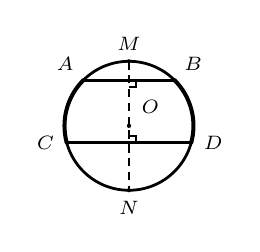
\begin{tikzpicture}[scale=0.39, every node/.style={font=\scriptsize, text=black}]
      \coordinate (O) at (0,0); \def\R{2.1}
      \coordinate (M) at (0,\R); \coordinate (N) at (0,-\R);
      \coordinate (A) at (135:\R); \coordinate (B) at (45:\R);
      \coordinate (C) at (195:\R); \coordinate (D) at (-15:\R);
      \coordinate (H1) at ($(A)!(O)!(B)$); \coordinate (H2) at ($(C)!(O)!(D)$);
      \draw[black, line width=1.0pt] (O) circle (\R);
      \draw[black, line width=1.05pt] (A)--(B) (C)--(D);
      \draw[black, line width=0.8pt, densely dashed] (M)--(N);
      \draw[black, line width=1.45pt] (A) arc (135:195:\R);
      \draw[black, line width=1.45pt] (D) arc (-15:45:\R);
      \draw[black, line width=0.6pt] ($(H1)+(0,-0.22)$)--($(H1)+(0.22,-0.22)$)--($(H1)+(0.22,0)$);
      \draw[black, line width=0.6pt] ($(H2)+(0,0.22)$)--($(H2)+(0.22,0.22)$)--($(H2)+(0.22,0)$);
      \fill[black] (O) circle (2pt) (M) circle (1.9pt) (N) circle (1.9pt) (A) circle (1.9pt) (B) circle (1.9pt) (C) circle (1.9pt) (D) circle (1.9pt);
      \node[above right=1pt] at (O) {$O$};
      \node[above=0.5pt] at (M) {$M$}; \node[below=0.5pt] at (N) {$N$};
      \node[above left=0pt] at (A) {$A$}; \node[above right=0pt] at (B) {$B$};
      \node[left=1pt] at (C) {$C$}; \node[right=1pt] at (D) {$D$};
    \end{tikzpicture}
  \end{minipage}
\end{tcolorbox}

\begin{tcolorbox}[
  enhanced, sharp corners, colback=white, colframe=black,
  boxrule=0.95pt, boxsep=2pt, top=3.2pt, bottom=3.2pt, left=6pt, right=6pt, after skip=3.8pt
]
  \begin{minipage}[c]{12.6cm}
    \textbf{២. លំហាត់ទី ៤ (ទំ.២០៤ — សំយោគពីជគណិត)៖} ក្នុងរង្វង់ $C(O,r)$ គេឱ្យ $OQ \perp AB,\; OR \perp CD$ និង $OQ = OR$។ បើ $AB = 6x + 14$ និង $CD = -4x + 4$ ចូរគណនាប្រវែង $AB$ និង $CD$៖
    \begin{itemize}[leftmargin=1.2em, itemsep=2pt, topsep=1.5pt]
      \item ដោយ $OQ \perp AB,\; OR \perp CD$ និង $OQ = OR$ តាមហេតុផលលេខ \blank{0.8cm} គេបាន៖ $AB =$ \blank{1.2cm}។
      \item ជំនួសកន្សោមពីជគណិត៖ $6x + 14 =$ \blank{2.2cm} $\Rightarrow 6x + 4x = 4 - 14 \Rightarrow 10x =$ \blank{1.2cm} $\Rightarrow x =$ \blank{1.1cm}។
      \item ផ្ទៀងផ្ទាត់ប្រវែង៖ $AB = 6($\blank{0.8cm}$) + 14 =$ \blank{1.1cm} និង $CD = -4($\blank{0.8cm}$) + 4 =$ \blank{1.1cm}។
    \end{itemize}
  \end{minipage}\hfill
  \begin{minipage}[c]{5.2cm}
    \centering
    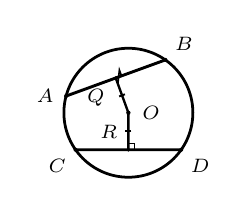
\begin{tikzpicture}[scale=0.39, every node/.style={font=\scriptsize, text=black}]
      \coordinate (O) at (0,0); \def\R{2.1}
      \coordinate (A) at (165:\R); \coordinate (B) at (55:\R);
      \coordinate (C) at (-145:\R); \coordinate (D) at (-35:\R);
      \coordinate (Q) at ($(A)!(O)!(B)$); \coordinate (R) at ($(C)!(O)!(D)$);
      \draw[black, line width=1.0pt] (O) circle (\R);
      \draw[black, line width=1.05pt] (A)--(B) (C)--(D);
      \draw[black, line width=0.85pt] (O)--(Q) (O)--(R);
      \draw[black, line width=0.6pt] ($(Q)!0.20cm!(B)$)--($(Q)!0.20cm!(B)!0.20cm!90:(B)$)--($(Q)!0.20cm!(O)$);
      \draw[black, line width=0.6pt] ($(R)+(0,0.20)$)--($(R)+(0.20,0.20)$)--($(R)+(0.20,0)$);
      \tickone{O}{Q}\tickone{O}{R}
      \fill[black] (O) circle (2pt) (A) circle (1.9pt) (B) circle (1.9pt) (C) circle (1.9pt) (D) circle (1.9pt) (Q) circle (1.8pt) (R) circle (1.8pt);
      \node[right=1.5pt] at (O) {$O$};
      \node[left=1pt] at (A) {$A$}; \node[above right=0pt] at (B) {$B$};
      \node[below left=0pt] at (C) {$C$}; \node[below right=0pt] at (D) {$D$};
      \node[below left=0.5pt] at (Q) {$Q$}; \node[above left=0.5pt] at (R) {$R$};
    \end{tikzpicture}
  \end{minipage}
\end{tcolorbox}

% ==================== ផ្នែកទី ៥ ៖ E5 - EVALUATE ====================
\secbar{ផ្នែកទី ៥ ៖ សម្រាយបញ្ជាក់ \enbf{Think-Pair-Share} និងបិទបេសកកម្ម (\enbf{E5 — Evaluate})}{\en{10} នាទី (ទំ.២០៣)}

\begin{tcolorbox}[
  enhanced, sharp corners, colback=white, colframe=black,
  boxrule=0.95pt, boxsep=2pt, top=3.2pt, bottom=3.2pt, left=6pt, right=6pt, after skip=3.8pt
]
  \begin{minipage}[c]{12.6cm}
    \textbf{១. ប្រតិបត្តិ (ទំ.២០៣ — គិតម្នាក់ឯង រួចពិភាក្សាដៃគូ)៖} ក្នុងរង្វង់ផ្ចិត $O$ មានអង្កត់ផ្ចិត $AD$ និងអង្កត់ធ្នូ $AB \parallel CD$ ដូចរូបខាងស្ដាំ។ ចូរស្រាយបញ្ជាក់ថា $AB = CD$៖
    \begin{itemize}[leftmargin=1.2em, itemsep=2pt, topsep=1.5pt]
      \item ដោយអង្កត់ធ្នូ $AB \parallel CD$ តាមលំហាត់គំរូទី ២ គេបានធ្នូចន្លោះ៖ $\arc{AC} =$ \blank{1.3cm}។
      \item ដោយ $AD$ ជាអង្កត់ផ្ចិត នោះកន្លះរង្វង់ទាំងពីរមានរង្វាស់ $180^\circ$៖ $\arc{AB} + \arc{BD} = 180^\circ$ និង $\arc{AC} + \arc{CD} = 180^\circ$។
      \item ទាញរក៖ $\arc{AB} = 180^\circ - \arc{BD} = 180^\circ -$ \blank{1.2cm} $=$ \blank{1.2cm}។ ដូចនេះ អង្កត់ធ្នូ \textbf{$AB =$ \blank{1.2cm}}!
    \end{itemize}
  \end{minipage}\hfill
  \begin{minipage}[c]{5.2cm}
    \centering
    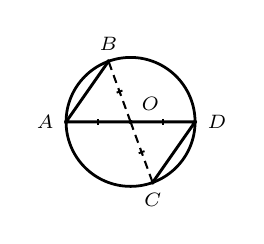
\begin{tikzpicture}[scale=0.39, every node/.style={font=\scriptsize, text=black}]
      \coordinate (O) at (0,0); \def\R{2.1}
      \coordinate (A) at (180:\R); \coordinate (D) at (0:\R);
      \coordinate (B) at (110:\R); \coordinate (C) at (-70:\R);
      \draw[black, line width=1.0pt] (O) circle (\R);
      \draw[black, line width=1.05pt] (A)--(D) (A)--(B) (C)--(D);
      \draw[black, line width=0.75pt, densely dashed] (O)--(B) (O)--(C);
      \tickone{O}{A}\tickone{O}{D}\tickone{O}{B}\tickone{O}{C}
      \fill[black] (O) circle (2pt) (A) circle (1.9pt) (B) circle (1.9pt) (C) circle (1.9pt) (D) circle (1.9pt);
      \node[above right=0.5pt] at (O) {$O$};
      \node[left=1pt] at (A) {$A$}; \node[right=1pt] at (D) {$D$};
      \node[above=0.5pt] at (B) {$B$}; \node[below=0.5pt] at (C) {$C$};
    \end{tikzpicture}
  \end{minipage}
\end{tcolorbox}

\begin{tcolorbox}[
  enhanced, sharp corners, colback=panelgray, colframe=black,
  boxrule=0.85pt, left=6pt, right=6pt, top=3pt, bottom=3pt, after skip=3.8pt
]
  \textbf{២. បិទបេសកកម្ម E1 (លូបេតុងមូល $r = 5\unit{dm},\; OH = 3\unit{dm}$)៖} ក្នុង $\tri{OHD}$ កែងត្រង់ $H$ តាមទ្រឹស្ដីបទពីតាករ \cnum{5}៖ $HD = \sqrt{OD^2 - OH^2} = \sqrt{5^2 - 3^2} =$ \blank{1.1cm} $\unit{dm}$។ តាម \cnum{3} ទទឹងផ្ទៃទឹកពេញគឺ $CD = 2 \times HD =$ \blank{1.2cm} $\unit{dm}$!\\[2.5pt]
  \textbf{៣. Exit Check (៦០ វិនាទី)៖} ក្នុងរង្វង់ $C(O, 10\unit{cm})$ អង្កត់ធ្នូ $AB$ ស្ថិតនៅចម្ងាយកែង $OH = 6\unit{cm}$ ពីផ្ចិត $O$។ តើប្រវែង $AB$ ស្មើប៉ុន្មាន?\\[1.5pt]
  \chkbox\ A. $8\unit{cm}$ \hspace{0.75cm} \chkbox\ B. $16\unit{cm}$ \hspace{0.75cm} \chkbox\ C. $12\unit{cm}$ \hspace{0.75cm} \chkbox\ D. $20\unit{cm}$
\end{tcolorbox}

% ==================== កិច្ចការផ្ទះសំយោគបញ្ចប់មេរៀនទី ១៥ ====================
\begin{tcolorbox}[
  enhanced, sharp corners, colback=white, colframe=black,
  boxrule=0.95pt, left=6pt, right=6pt, top=3.2pt, bottom=3.2pt
]
  {\muol\fontsize{9.4pt}{13.8pt}\selectfont កិច្ចការផ្ទះសំយោគបញ្ចប់មេរៀនទី១៥ ៖ រង្វង់ (សៀវភៅសិក្សាគោល ទំព័រ ២០៤)}\\[2pt]
  $\bullet$ \textbf{លំហាត់ទី ៨ (ទំ.២០៤)៖} កន្លះរង្វង់ផ្ចិត $O$ មានអង្កត់ផ្ចិត $AB$ និងអង្កត់ធ្នូ $CD$។ គេគូស $AP \perp CD$ ត្រង់ $P$ និង $BS \perp CD$ ត្រង់ $S$។ ចូរបង្ហាញថា $PC = DS$ \textit{(ណែនាំ៖ គូស $OH \perp CD$ ត្រង់ $H$ នោះ $HC = HD$ ហើយ $OH$ ជាអង្កត់មធ្យមនៃចតុកោណព្នាយកែង $ABSP \Rightarrow HP = HS$)}។\\[1.8pt]
  $\bullet$ \textbf{លំហាត់ទី ៩ (ទំ.២០៤)៖} យកចំណុច $P$ មួយនៅក្នុងរង្វង់ $C(O,r)$ ($P \neq O$)។ ចូរបង្ហាញថាអង្កត់ធ្នូដែលកាត់តាម $P$ ហើយកែងនឹង $OP$ មានប្រវែងខ្លីជាងគេក្នុងចំណោមអង្កត់ធ្នូទាំងអស់ដែលកាត់តាម $P$។\\[1.8pt]
  $\bullet$ \textbf{លំហាត់ទី ១០ (ទំ.២០៤ — សម្រាប់សិស្សពូកែ)៖} ក្នុងរង្វង់ $C(O,r)$ អង្កត់ធ្នូ $AB > CD$ កាត់គ្នាត្រង់ $K$ នៅក្រៅរង្វង់ ($H, P$ ជាចំណុចកណ្ដាលនៃ $AB, CD$ និង $M$ ជាចំណុចកណ្ដាលនៃ $OK$)។ បង្ហាញថា៖ (ក) $MO = MK = MH = MP$, (ខ) $\angle HKO < \angle PKO$, និង (គ) $KH > KP$។
\end{tcolorbox}

\end{document}
